\newcommand{\svcourse}{CST Part IA: Software Engineering and Security}
\newcommand{\svnumber}{1}
\newcommand{\svvenue}{Microsoft Teams}
\newcommand{\svdate}{2022-05-11}
\newcommand{\svtime}{15:00}
\newcommand{\svuploadkey}{CBd13xmL7PC1zqhNIoLdTiYUBnxZhzRAtJxv/ytRdM1r7qIfwMsxeVwM/pPcIo8l}

\newcommand{\svrname}{Dr Sam Ainsworth}
\newcommand{\jkfside}{oneside}
\newcommand{\jkfhanded}{yes}

\newcommand{\studentname}{Harry Langford}
\newcommand{\studentemail}{hjel2@cam.ac.uk}


\documentclass[10pt,\jkfside,a4paper]{article}

% DO NOT add \usepackage commands here.  Place any custom commands
% into your SV work files.  Anything in the template directory is
% likely to be overwritten!

\usepackage{fancyhdr}

\usepackage{lastpage}       % ``n of m'' page numbering
\usepackage{lscape}         % Makes landscape easier

\usepackage{verbatim}       % Verbatim blocks
\usepackage{listings}       % Source code listings
\usepackage{graphicx}
\usepackage{float}
\usepackage{epsfig}         % Embed encapsulated postscript
\usepackage{array}          % Array environment
\usepackage{qrcode}         % QR codes
\usepackage{enumitem}       % Required by Tom Johnson's exam question header

\usepackage{hhline}         % Horizontal lines in tables
\usepackage{siunitx}        % Correct spacing of units
\usepackage{amsmath}        % American Mathematical Society
\usepackage{amssymb}        % Maths symbols
\usepackage{amsthm}         % Theorems

\usepackage{ifthen}         % Conditional processing in tex

\usepackage[top=3cm,
            bottom=3cm,
            inner=2cm,
            outer=5cm]{geometry}

% PDF metadata + URL formatting
\usepackage[
            pdfauthor={\studentname},
            pdftitle={\svcourse, SV \svnumber},
            pdfsubject={},
            pdfkeywords={9d2547b00aba40b58fa0378774f72ee6},
            pdfproducer={},
            pdfcreator={},
            hidelinks]{hyperref}

\renewcommand{\headrulewidth}{0.4pt}
\renewcommand{\footrulewidth}{0.4pt}
\fancyheadoffset[LO,LE,RO,RE]{0pt}
\fancyfootoffset[LO,LE,RO,RE]{0pt}
\pagestyle{fancy}
\fancyhead{}
\fancyhead[LO,RE]{{\bfseries \studentname}\\\studentemail}
\fancyhead[RO,LE]{{\bfseries \svcourse, SV~\svnumber}\\\svdate\ \svtime, \svvenue}
\fancyfoot{}
\fancyfoot[LO,RE]{For: \svrname}
\fancyfoot[RO,LE]{\today\hspace{1cm}\thepage\ / \pageref{LastPage}}
\fancyfoot[C]{\qrcode[height=0.8cm]{\svuploadkey}}
\setlength{\headheight}{22.55pt}


\ifthenelse{\equal{\jkfside}{oneside}}{

 \ifthenelse{\equal{\jkfhanded}{left}}{
  % 1. Left-handed marker, one-sided printing or e-marking, use oneside and...
  \evensidemargin=\oddsidemargin
  \oddsidemargin=73pt
  \setlength{\marginparwidth}{111pt}
  \setlength{\marginparsep}{-\marginparsep}
  \addtolength{\marginparsep}{-\textwidth}
  \addtolength{\marginparsep}{-\marginparwidth}
 }{
  % 2. Right-handed marker, one-sided printing or e-marking, use oneside.
  \setlength{\marginparwidth}{111pt}
 }

}{
 % 3. Alternating margins, two-sided printing, use twoside.
}


\setlength{\parindent}{0em}
\addtolength{\parskip}{1ex}

% Exam question headings, labels and sensible layout (courtesy of Tom Johnson)
\setlist{parsep=\parskip, listparindent=\parindent}
\newcommand{\examhead}[3]{\section{#1 Paper #2 Question #3}}
\newenvironment{examquestion}[3]{
\examhead{#1}{#2}{#3}\setlist[enumerate, 1]{label=(\alph*)}\setlist[enumerate, 2]{label=(\roman*)}
\marginpar{\href{https://www.cl.cam.ac.uk/teaching/exams/pastpapers/y#1p#2q#3.pdf}{\qrcode{https://www.cl.cam.ac.uk/teaching/exams/pastpapers/y#1p#2q#3.pdf}}}
\marginpar{\footnotesize \href{https://www.cl.cam.ac.uk/teaching/exams/pastpapers/y#1p#2q#3.pdf}{https://www.cl.cam.ac.uk/\\teaching/exams/pastpapers/\\y#1p#2q#3.pdf}}
}{}


\usepackage{graphicx}
\usepackage{float}
\usepackage{wasysym}
\usepackage{color}

\begin{document}

\begin{examquestion}{1997}{5}{5}

A slightly clumsy programmer had been lagging behind the company
productivity targets and needed to write some C++ code in a hurry. Almost
remembering an old optimising compilers question from student days, this
programmer produced a file containing the test:

\begin{lstlisting}[language=C, numbers=left]
struct List {int head; struct list *tail};

struct List readlist(){
	int i;
	struct List *p, *q, *t;
L1:	p = NULL;
L2:	while (scanf("%d", i) = 1)
	/* scanf reads an integer and returns 1
		if it finds one correctly /*
	[
L3:		t = malloc(sizeof(List *));
		if (t == 0) printf("oops no memery\n");
		else t->hd = i;
L4:			 t->tl = 0;
		if (p == NULL)
			p = q = t;
		else
			q->tl = t, q = t;
	}
L5:	return p;
}

\end{lstlisting}

Unfortunately the programmer had forgotten what this was supposed to
achieve; you are asked to help re-create an explanation for the code and to
identify problems (of either style or correctness) in it. You do not need to
provide a correct version of the program: just draw attention to as many
errors or oddities as you can.

The errors and oddities in this code are as follows:

\begin{itemize}

\item Firstly, the code is ``written in C++'' however uses none of the
features of C++, employing only C. This defeats the purpose of writing in
C++ and is completely against convention.

\item On line 1:

When declaring \texttt{struct List}, second field has type \texttt{struct list
*} rather than \texttt{struct List *}. This is not a valid type and so would
cause a compile error.

The fields of \texttt{struct List} are \texttt{head} and \texttt{tail}.
However, they are consistently referred to as \texttt{hd} and \texttt{tl} in
the code. So either the fields should be called \texttt{hd} and \texttt{tl}
or the rest of the code should be refactored to refer to the fields as
\texttt{head} and \texttt{tail}. These name errors are a compile time error.
Additionally, both fields are declared on one line -- which makes it harder
to read.

When declaring structs it is good practice to typedef to give the struct a
better name and simplify later code. This is not done in this program and is
an oddity.

\item On line 3:

The function \texttt{readlist()} has a return type of \texttt{struct List} --
but the return type is actually of type \texttt{struct List *}. This would
cause a compile error.

\texttt{readlist()} also has the wrong type signature. \texttt{()} means
readlist may take any number of parameters of unknown types. It should
instead be called \texttt{readlist(void)} to take no parameters. As declared,
users could pass any number of arguments to readlist and there would be no
compile time error. Therefore declarations with \texttt{()} are strongly
discouraged. If this code is compiled in C++ then this is not an issue --
but there is some ambiguity about which language this code is actually
compiled in and so this \textit{could} be a problem.

\item On lines 4 \& 5:

The variable names have no meaning -- this is poor programming practice and
makes the program harder to understand.

It is better practice to only declare variables for the scope in which they
are used. \texttt{t} is only used inside the while loop -- it would therefore
be better practice to declare it inside the while loop -- it is an oddity to
declare it outside. However, historically it was considered good practice to
declare variables at the start of a function and was defined in the C
standard at one point. I don't know whether this has \textit{become} an
oddity or whether it was initially intended as one.

\item On line 6:

The program uses labels throughout despite the fact that it never uses
goto to jump to those labels. This just clutters up the program and makes it
more difficult to read. I'm not suggesting the use of goto in this program --
only stating that the only reason to use labels in C is if you are going to
use goto. Labels are used on lines 6, 7, 11, 14 \& 20. I will not repeat
this oddity.

\item On line 7:

\texttt{scanf} is provided by the ``stdio.h'' header -- which has not been
included in the program. This will cause a compile error.

\texttt{scanf} requires a pointer to the variable we wish to update -- not
just it's value -- which is what is being passed. This means the call should be
\texttt{scanf("\%d", \&i)}. Passing an integer to scanf will cause a compile
error.

The programmer is using the assignment operator \texttt{=} rather than equality
\texttt{==}. So this attempts to assign the value 1 to a function call. This
is a compile error.

\texttt{scanf} will return 0 if it fails. It returns 1 if it successfully
assigns an integer to i. It is more elegant therefore for the condition to
be \texttt{while (scanf("\%d", \&i))} without an equality test. Having an
equality test is an oddity.

{\color{blue} What if the return value is a 0 or 1?}

{\color{blue} If \texttt{scanf} fails to read then it may throw an error code
-- which may be an almost random number. Therefore on failure, \texttt{scanf} can
return an non-zero value ie -1}

There is no message informing the user what they should be inputting.
Whether or not this is necessary depends on the context. However, it felt
worth mentioning.

There is no obvious way to exit this while loop without error. Inputting
``$\backslash$'' will gracefully escape the loop, however this is not conveyed
to the user either when executing or in the source code. This is a usability
failure.

\item On line 8:

This is likely personal, but it feels incorrect and certainly odd to have a
comment between a \texttt{while} and the while block.

{\color{blue} Not that odd}

\item On line 9:

The multiline comment ends with \texttt{/*} -- it should end with \texttt{*/}.
This means the comment is not ended -- the rest of the program will be
commented out. This will cause a compile error.

The comment is ambiguous -- does scanf return \texttt{1} if it finds an integer
correctly or if the integer is \texttt{1}?

\item On line 10:

The block is opened with \texttt{[} rather than \texttt{\{}. This is a compile error.

\item On line 11:

\texttt{malloc} is implemented in the ``stdlib.h'' header -- which has not been
included in the program. This can be resolved with \texttt{\#include <stdlib.h>}.
The lack of inclusion would cause a compile error.

The call allocates a pointer to a \texttt{List *} which will be allocated on
the heap. \texttt{List *} is not a valid type -- this is a compile error -- the
programmer means to allocate a struct \texttt{List *}. Secondly, allocating a
pointer to a \texttt{struct List *} is a logic error. We should instead allocate
a \texttt{struct List}.

\item On line 12:

\texttt{t == 0} compares a pointer to an integer. This will raise a warning.
It would be better to compare to \texttt{NULL} -- however checking for
\texttt{t == NULL} is odd. It would be more elegant for the comparison to be
\texttt{if (t)} and to swap the if and else clauses.

The error message given is uninformative and almost joking. This is an
unhelpful message. Additionally there is a typo in the message.

After the out of memory exception is noticed, it is never addressed. This
would be a suitable time for the function to exit or an error handling
routine to start.

Additionally, whether printf allocates memory is unspecified. So in some
implementations, printf may need to allocate heap memory -- however, we've
just run out of heap space. Meaning that the call to \texttt{printf} may
fail. There is no obvious way to resolve an out of memory exception and the
best approach is case specific. For example Java allocates the
\texttt{OutOfMemoryException} object on startup and raises it on failure. I
think the best approach in this situation would be to return or free the
last few nodes of the list.

\item On line 13:

The programmer has not put a braces around the body of the else clause.
This means that the else clause only contains only \texttt{t->hd = i}. The
\texttt{t->tl = 0} is outside the clause. Since t could be NULL, this may lead to
dereferencing a null pointer.

\item On line 14:

The tl attribute of struct List is of type \texttt{struct List *}. However
we assign an integer to it. This is a warning and instead we should assign
\texttt{NULL} .

\item On line 15:

if \texttt{p == NULL} is unnecessarily verbose. It would be better practice
to swap the if and else clauses and have the condition as ``if (p)''.

\item On line 18:

An oddity is that the  else clause has two different expressions separated
by a \texttt{,}. However, the return type is not used. It is therefore better
practice to separate them by \texttt{;} -- it's clearer and does not change the
meaning.

\end{itemize}

This code is meant to read in a stream of integers and build a linked list
containing those integers.

A correct implementation in C is below:

\begin{lstlisting}[language=C]

#include <stdlib.h>
#include <stdio.h>

typedef struct List* list;

struct List {
	int value;
	list next;
};

list readlist(void){
	int i;
	list head = NULL, current = NULL;
	printf("Input the elements of the integer linked list\n")
	while (scanf("%d", &i)){
		list temp = malloc(sizeof(struct List));
		if (temp){
			temp->value = i;
			temp->next = NULL;
		}
		else{
			/*
			error routine for out of memory exception
			I would need more information to know what
			would be most appropriate.
			possible routines would include:
			return current list,
			write current list to a file,
			deallocate head of the list to make space,
			deallocate the whole list
			...
			*/
		}
		if (head){
			current->value = temp;
			current = temp;
		}
		else{
			head = current = temp;
		}
	}
	return head;
}

\end{lstlisting}

Suggest two ways in which a move from C to C++ might allow the structure of
the code to be improved.

C++ has classes. This would allow all methods related to the Linked List to
be encapsulated in a single class. This would remove the need for a separate
``struct'' and allow us to neatly organise and contain all code relating to
the Linked List in a sigle file. This would also allow a level of
abstraction -- the end-user would not need to know how the linked list works
to use it. Implementing the Linked List in this way would also allow us to
manage it better, preventing it becoming cyclic or leaking.

C++ also provides exceptions, this would allow better management of the
OutOfMemoryException that could be caused by repeatedly allocating onto the
heap.

C++ also has more intuitive memory management. Allocating objects on the heap
only requires the keyword ``new'' and removing it uses only the keyword delete.
The programmer will no longer have to use sizeof operator which will make
the code neater.

\end{examquestion}

\begin{examquestion}{2007}{3}{4}

A C programmer is working with a little-endian  machine with 8 bits in a 
byte and 4 bytes in a word. The compiler supports unaligned access and uses 
1, 2 and 4 bytes to store char, short and int respectively. The programmer 
writes the following definitions (below right) to access values in main 
memory (below left):

\begin{figure}[H]
    \centering
    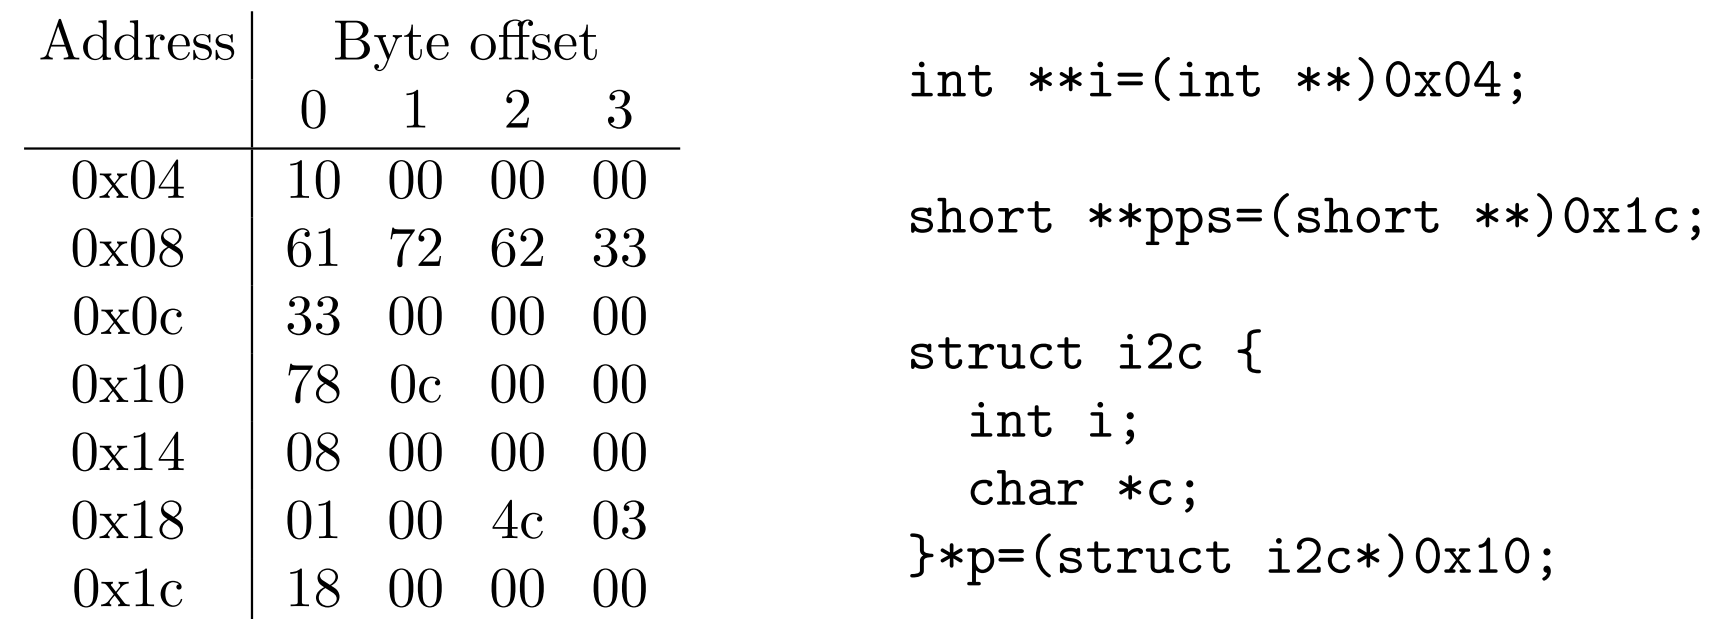
\includegraphics[width=0.8\textwidth]{q2_img}
\end{figure}

\begin{enumerate}[label=(\alph*)]

\item Write down the values for the following C expressions:

\begin{align*}
**i & & p\rightarrow c[2] & & \&(*pps)[1] & & ++p\rightarrow i
\end{align*}

\begin{itemize}

\item $**i$ has value $3192$ of type int.

$i$ is a pointer to $0x04$. So $*i$ returns the value stored at $0x04$.
Which is the address $0x10$. $**i$ returns the value stored at $0x10$ --
which is $12 \cdot 16^2 + 7\cdot 16 + 8 = 3192$.

\item $p\rightarrow c[2]$ has value `J' of type char.

$p\rightarrow c[2]$ is the dereference of the address of the $c$ attribute of
$p$ plus two bytes (as a char in C is 1 byte). $p$ is the struct i2c with
memory starting at 0x10. The $i$ attribute is 4 bytes. So the $c$ attribute
is a pointer stored at $0x14$. This can be viewed as an array starting at
the address $0x08$. $p\rightarrow c[2]$ is the second element of
this array. Since chars have size 1 byte, the second element of this array
is at address $0x10$ -- which has value $0x62$ (`J').

\item $\&(*pps)[1]$ is a pointer of type $short *$ to $0x1a$.

*pps first dereferences $pps$. This is a pointer to $0x18$. $*pps$ has type
$*short$ -- which can be viewed as an array of shorts. $[1]$ finds the
second element in this array. This can be done by adding the size of a short
to the address $*pps$. Shorts in C are two bytes. Therefore the address of
$(*pps)[1]$ is $0x1a$. So $\&(*pps)[1]$ is a pointer to $0x1a$ and is of
type short*.

\item $++p\rightarrow i$ has value $3193$ and is of type int.

This accesses the $i$ element of $p$, increments it and returns the
incremented value. The $i$ attribute of $p$ is stored at address 0x10. This
has value $3192$. So we increment this by one and return the incremented value.
Therefore this expression has value 3193 and type int.

\end{itemize}

\item Explain why the code shown below, when executed will print the value 420.

\begin{lstlisting}[language=C, numbers=left]
#include <stdio.h>

#define init_employee(X,Y) {(X),(Y), wage_emp}
typedef struct Employee Em
struct Employee {int hours, salary; int (*wage) (Em*);};
int wage_emp(Em *ths) {return ths->hours*ths->salary;}

#define init_manager(X,Y,Z) {(X),(Y),wage_man,(Z)}
typedef struct Manager Mn;
struct Manager {int hours,salary;int (*wage)(Mn*);int bonus;};
int wage_man(Mn *ths){return ths->hours*ths->salary+ths->bonus;}

int main(void){
	Mn m = init_manager(40,10,20);
	Em *e= (Em *) &m;
	printf("%d\n",e->wage(e));
	return 0;
}
\end{lstlisting}

The datatype Em has fields hours, salary and a function pointer
(the function pointer is called wage -- the function is not necessarily
called wage) pointing to a function that takes an argument of type Em* and
returns an integer. Mn is the same but with two differences: the
function takes argument of type Mn and there is an additional
field ``bonus''.

\#define is used to define macros in the C preprocessor.
The first argument will be replaced by the second argument.

The two macros on lines 3 \& 8 tell the C preprocessor to replace all
occurrences of init\_employee and init\_manager in the rest of the program
with initialisers for the respective structs. This means init\_employee and
init\_manager now function as initialisers.

Therefore \texttt{Mn m = init\_manager(40, 10, 20);} (line 14) will initialise
a struct of type manager on the stack who works 40 hours at salary 10 with a
bonus of 20.

On line 15, we create a pointer \texttt{e} of type \texttt{Em *} to this
object -- this requires an unsafe cast. C is not strongly typed and so this
is allowed.

In C, attributes of structs are accessed only by offset. So the attempt to
access the wage function pointer of \texttt{e} will access the bits at offset
\texttt{2 * sizeof(int)}. Since the first fields of \texttt{Mn} are the same
as the first fields of \texttt{Em}; the offset for the function pointer of
\texttt{Mn} is the same as the offset for the function pointer of \texttt{Em}.
Therefore \texttt{e->wage} will access the function pointer of \texttt{m}.
This is a pointer to the \texttt{wage\_man} function. This is then passed
\texttt{e}. \texttt{e} is interpreted by the function \texttt{wage\_man} as
being of type \texttt{Mn}. This is the same as passing a pointer to \texttt{m}
to \texttt{wage\_man}. Therefore the return value of the function call is
$40*10 + 20 = 420$. This is then passed to \texttt{printf} -- therefore the
program outputs 420 as required.

\end{enumerate}

\end{examquestion}

\begin{examquestion}{2010}{3}{6}

\begin{enumerate}[label=(\alph*)]

\item Popular programming journal \textit{Obscure C Techniques for Experts}
has published a novel way to save space for a doubly-linked list program.
Instead of storing two pointers (one next and one previous), this new
technique stores a single value: the XOR of \textit{previous} and
\textit{next} pointers.

A traditional two-pointer linked list might be illustrated as:
\begin{table}[H]
\centering
\begin{tabular}{c c c c c c c c c c c}
\dots & A & & B & & C & & D & & E & \dots \\
& & $\longrightarrow$ & next & $\longrightarrow$ & next & $\longrightarrow $
 & next & $\longrightarrow $ \\
& & $\longleftarrow$ & prev & $\longleftarrow$ & prev & $\longleftarrow $
 & prev & $\longleftarrow $ \\
\end{tabular}
\end{table}

In contrast, the proposed new technique stores a bit-wise XOR of the
\textit{previous} and \textit{next} pointers within a single field.

\begin{table}[H]
\centering
\begin{tabular}{c c c c c c c c c c c}
\dots & A & & B & & C & & D & & E & \dots \\
& & $\longleftrightarrow $ & $\oplus$ & $\longleftrightarrow $ & $\oplus $ &
 $\longleftrightarrow $ & $\oplus $ & $\longleftrightarrow $ \\
\end{tabular}
\end{table}

You have been engaged to provide code examples of this approach for
publication.

Ensure your code illustrates the creation and initialisation of such a list
as well as the insertion, and deletion of elements from such a list.
Additionally, you must provide examples of a forward or backward traversal
of the list permitting combination of each element in turn.

\begin{lstlisting}[language=C]

#include <stdlib.h>

typedef struct List * list;

struct List {
	int value;
	list xorpntr;
};

list create_list(int head_value){
	list lst = malloc(sizeof(struct List));
	lst->value = head_value;
	// NULL ^ NULL = NULL
	lst->xorpntr = NULL;
	return lst;
}

void free_list(*list lst){
	// check for NULL
	if (!lst) return;
	/*
	The while condition is true until both pointers are equal
	The linked list is not cyclic so the pointers should only
	be equal when both are NULL -- when we're on the last node
	*/
	while (lst->xorpntr){
		/*
		if one pointer is NULL, xorpntr is the
		value of the other pointer.
		This updates the next nodes xorpntr
		*/
		lst->xorpntr->xorpntr ^= lst;
		list prev = lst;
		lst = lst->xorpntr;
		free(prev);
	}
	free(lst);
}

void addfirst(list *lst, int val){
	list fst = malloc(sizeof(struct List));
	fst->value = val;
	fst->xorpntr = *lst;
	(*lst)->xorpntr ^= fst;
	*lst = fst;
}

void addlast(list lst, int val){
	list current = lst;
	list next = current->xorpntr;
	// if there is only one element in the list
	if (!next){
		list last = malloc(sizeof(struct List));
		current->xorpntr = last;
		last->xorpntr = NULL;
		last->value = val;
		return;
	}
	// while ends when next is the last element in the list
	while (next->xorpntr != current){
		list tmp = next;
		next = next->xorpntr^current;
		current = tmp;
	}
	list last = malloc(sizeof(struct List));
	last->value = val;
	last->xorpntr = next;
	next->xorpntr = current^last;
}

int popFirst(list *lst){
	// check for NULL
	if (!lst) return 0;
	// this works for list of length 1+
	int i = (*lst)->value;
	list tmp = *lst;
	*lst = (*lst)->xorpntr;
	free(*lst);
	return i;
}

int popLast(list *lst){
	// check for NULL
	if (!(*lst)) return 0;
	// check for list of length 1
	if (!(*lst)->xorpntr){
		int i = (*lst)->value;
		free(*lst);
		*lst = NULL;
		return i;
	}
	int current = *lst;
	int next = current->xorpntr;
	/*
	Terminates when next is the last node and
	current is the penultimate node
	*/
	while (next->xorpntr != current){
		current = next;
		next = next->xorpntr;
	}
	int i = next->value;
	// update penultimate pointer
	current->xorpntr ^= next;
	// free last node
	free(next);
	return i;
}

\end{lstlisting}

\item Comment on this form of linked list. Consider the comparative speed,
memory overheads and maintenance and other advantages or disadvantages of
the XOR doubly-linked list approach when compared with an approach that
stores both \textit{previous} and \textit{next} pointers.

The primary advantage of the XOR list is that it requires less memory. Each
node now only requires one pointer (size) rather than two. This will reduce
the size of the linked list structure significantly -- especially in C as
structs have no additional information. In a memory-critical system this
could be a significant advantage.

However, iterating through the XOR list is more complicated and slower.
Rather than just looking up a value (which will likely already be in cache),
we've got to perform an XOR operation which will double the amount of
machine instructions. I'd like to note that iterating through a linked list
is dominated by memory accesses rather than cpu time -- so this will not
double the time; just increase it. Additionally, the programmer has to do
more work, will write code that is more difficult to understand and less
intuitive. This increases the probability of a bug which could lead to
accessing unallocated memory or dereferencing a \texttt{NULL} pointer.

Furthermore, it's much harder implement cyclical linked lists in the XOR list
or incorporate it into larger data structures. If we pass a reference to a
node in the linked list, we cannot use it. We need two nodes to iterate in
one direction -- in the base case we know one pointer is NULL and so can
iterate that in the other direction. Therefore to use the XOR list in a
cyclical linked list, we need to pass two nodes which adds extra work to
external methods and breaks encapsulation. If we want to use the XOR list
in another structure such as a Fibonacci Heap, then we will have to hold
the node and an adjacent node -- which doubles the space requirement for
the linked list in the fibonacci heap -- which cancels out the memory gain
in the XOR list itself. Therefore there is no reason to use the XOR list in
another more complicated data structure.

\end{enumerate}

\end{examquestion}

\begin{examquestion}{2014}{3}{3}

\begin{enumerate}[label=(\alph*)]

\item Write a C function revbits() which takes a single 8-bit char parameter
and returns a char result by reversing the order of the bits in the char.

\begin{lstlisting}[language=C]

char revbits(char c){
	char x = 0;
	int j = 128;
	for (int i = 1; i <= 128; i *= 2, j /= 2){
		if (c & i) {
			x |= j;
		}
	}
	return x;
}

\end{lstlisting}

\item Write a C function revbytes() taking two parameters and returning no
result. The first parameter is a pointer to memory containing $n$ contiguous
bytes (each of type char), and the second is the number of bytes. The
function should have the side effect of reversing the order of the bits in
the $n$ contiguous bytes, seen as a bitstring of length $8n$. For example
the first bit of the first char should be swapped with the last bit of the
last char.

\begin{lstlisting}[language=C]

void revbytes(char *mem, int n){
	int lo = 0;
	int hi = n - 1;
	while (lo < hi){
		char tmp = revbits(mem[lo]);
		mem[lo++] = revbits(mem[hi]);
		mem[hi--] = tmp;
	}
	if (n % 2) {
		mem[n / 2] = revbits(mem[n / 2];
	}
}

\end{lstlisting}

\end{enumerate}

\end{examquestion}

\end{document}
